\documentclass[conference]{IEEEtran}
\usepackage{times}

\usepackage[numbers]{natbib}
\usepackage{multicol}
\usepackage[bookmarks=true]{hyperref}
\usepackage{amsmath}
\usepackage{graphicx}
\usepackage{tikz}
\usepackage{tikzducks}

\pdfinfo{
   /Author (Anonymous)
   /Title  (Learning Uncertainty for Generalizable Vision--Inertial Spatial Perception)
   /Subject (RSS Pioneers Research Statement)
   /Keywords (SLAM; uncertainty; visual-inertial odometry; spatial perception)
}

\begin{document}

\title{Learning Uncertainty for Generalizable Vision--Inertial Spatial Perception}

\author{Author Names Omitted for Anonymous Review.}

\maketitle

\begin{figure}[t]
  \centering
  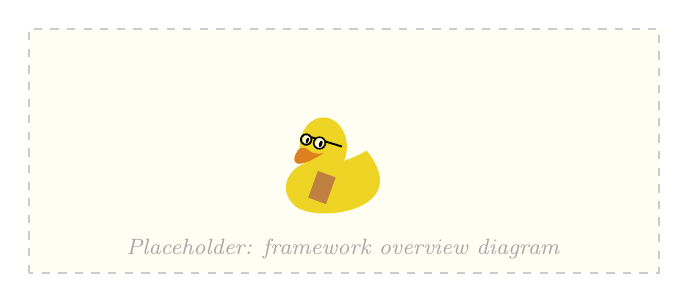
\begin{tikzpicture}
    \fill[yellow!5] (-0.5,-0.3) rectangle (7.5,2.8);
    \draw[thick, gray!40, dashed] (-0.5,-0.3) rectangle (7.5,2.8);
    \duck[xshift=2.7cm, yshift=0.4cm, scale=0.6, glasses, book]
    \node[gray!70] at (3.5, 0) {\footnotesize\textit{Placeholder: framework overview diagram}};
  \end{tikzpicture}
  \caption{Learned uncertainty as the unifying principle for vision--inertial spatial perception.
  Metrics-aware covariance learned from visual and inertial data drives
  principled fusion, cross-platform generalization, and compute-efficient deployment,
  advancing toward spatial perception for any robot, anywhere.}
  \label{fig:overview}
\end{figure}

\section{Introduction}

Autonomous robots must perceive and localize reliably across diverse platforms, sensors, and operating conditions---from handheld devices to aerial vehicles, indoors to outdoors, day to night.
The ultimate goal of spatial perception is a system that works for \textit{any robot, anywhere}, without manual tuning.
Yet despite decades of progress in simultaneous localization and mapping (SLAM) and visual-inertial odometry (VIO), current systems remain brittle when deployed beyond their calibrated settings~\cite{forster2015imu, qin2018vins}.

A central cause of this brittleness is the treatment of measurement uncertainty.
Classical SLAM pipelines model sensor noise with hand-tuned, fixed covariance matrices that assume stationary Gaussian distributions~\cite{forster2015imu, qin2018vins}.
These parameters cannot capture environment-dependent sensor reliability---a stereo camera calibrated indoors produces overconfident estimates in outdoor lighting, and an IMU noise model tuned on a ground vehicle fails on an aerial platform with different vibration characteristics.
Consequently, deploying a perception system on a new robot or in a new environment requires extensive per-platform recalibration by domain experts, a process that does not scale to the diversity of robots and conditions encountered in real-world autonomy.

Learning-based odometry methods have demonstrated strong accuracy in recent years~\cite{teed2021droid}, yet they typically produce scale-agnostic confidence weights that do not reflect actual estimation error in metric space.
This lack of calibrated, metrics-aware uncertainty limits their integration into multi-sensor fusion, prevents reliable failure detection, and makes downstream planning and control fragile.
Meanwhile, efficiency-oriented quantization methods~\cite{frantar2022gptq} target general network acceleration but do not account for the geometry-aware structure unique to perception pipelines.

My research addresses these limitations by developing \textbf{learned uncertainty} as the unifying principle for generalizable, robust, and efficient vision--inertial spatial perception.
Rather than treating uncertainty as a fixed parameter, I learn it from data as a \textit{metrics-aware, calibrated belief} that transfers across cameras, IMUs, platforms, and conditions.
This learned uncertainty enables three tightly coupled capabilities:
(i)~principled multi-modal fusion through calibrated measurement weighting,
(ii)~robustness via explicit knowledge of when and where perception is reliable, and
(iii)~system acceleration through uncertainty-guided, compute-efficient inference that allocates resources where they matter most.

\section{Past and Current Research}

My research develops learned uncertainty for each sensing modality, accelerates perception for edge deployment, and fuses the components into a robust visual-inertial system.
Concretely, I first learn metrics-aware visual uncertainty to select correspondences and weight optimization without hand tuning.
I then learn inertial uncertainty propagation and observability-aware inertial representations that transfer across IMUs and platforms.
To make these models usable on real robots, I develop uncertainty-guided compression and acceleration for edge hardware.
Finally, I bring the learned components together in tuning-free visual-inertial initialization and calibration, using uncertainty as the common currency that makes fusion principled and reliable.

\subsection{Metrics-Aware Stereo Visual Odometry}

We developed a stereo visual odometry system~\cite{anonymous2025macvo} that learns to predict metrics-aware covariance directly from visual features, replacing hand-tuned geometric noise models.
Unlike the scale-agnostic diagonal confidence weights used by prior learning-based methods~\cite{teed2021droid}, our system introduces two innovations: a learning-based model that quantifies 2D matching uncertainty by reasoning over appearance, context, and occlusion cues, and a novel covariance propagation scheme that lifts these 2D uncertainties into full 3D covariance (including inter-axis correlations) via the stereo geometry.
The resulting metrics-aware covariance serves a dual role: it drives keypoint selection by filtering unreliable correspondences and weights residuals in the two-frame pose graph optimization proportional to each measurement's actual reliability.
Without any manual tuning, this two-frame system outperforms existing VO algorithms and even multi-frame SLAM systems on public benchmarks across diverse cameras and conditions.

\subsection{Data-Driven Inertial Odometry and Uncertainty Propagation}

IMU preintegration traditionally relies on fixed white-noise parameters that cannot capture platform-specific vibration, bias drift, or motion-dependent stochastic errors.
We developed a data-driven framework~\cite{anonymous2025airimu} that jointly learns to correct raw IMU measurements and propagate the resulting uncertainty through a fully differentiable preintegration pipeline.
Rather than replacing the kinematic model with a black-box network, the approach preserves the classical preintegration structure while learning a residual noise correction and a covariance propagation function that captures platform- and motion-specific noise patterns.
Building on this, we proposed an inertial odometry system~\cite{anonymous2025airio} that addresses a complementary challenge: limited observability of certain motion states under constrained dynamics.
The system enhances IMU feature representations to improve state observability and combines learned uncertainty with robust estimation, achieving significantly reduced drift in long-trajectory, GPS-denied environments such as subterranean and aerial operations.

\subsection{Compute-Efficient Perception Deployment}

Learned perception models impose heavy computational demands that limit deployment on edge devices carried by real robots.
We addressed this challenge on two fronts.
First, we developed a full-stack quantization framework for learning-based VO with metrics-aware covariance~\cite{anonymous2026quantmacvo}: a sim-to-real calibration strategy on synthetic data enables zero-shot generalization, and a kurtosis-based hybrid quantization scheme selectively applies expensive rotations only to outlier-dominated layers, achieving $1.83\times$ speedup on NVIDIA Jetson Thor with negligible accuracy loss.
Second, we introduced confidence-guided token merging~\cite{anonymous2026come} for visual geometry transformers, where a lightweight predictor ranks tokens by uncertainty and selectively merges uninformative ones, yielding up to $11.3\times$ speedup for dense 3D reconstruction and $7.2\times$ for semantic mapping on edge hardware.

\subsection{Tuning-Free Visual-Inertial Initialization}

We designed a robust VI initialization and online calibration system~\cite{anonymous2026macinit} that leverages metrics-aware uncertainty from both the visual and inertial modules.
Traditional VI initialization fails under extreme exposure, textureless scenes, or dynamic objects because it relies on manually set noise parameters that cannot reflect actual measurement quality.
By deriving visual pose covariance from learned feature-matching uncertainty and inertial covariance from the learned preintegration model, our system formulates a principled initialization that weights visual and inertial constraints according to their true reliability.
This removes the manual parameter adjustment that typically accompanies each new platform, achieving tuning-free initialization across diverse environments and sensor configurations.

\begin{figure}[t]
  \centering
  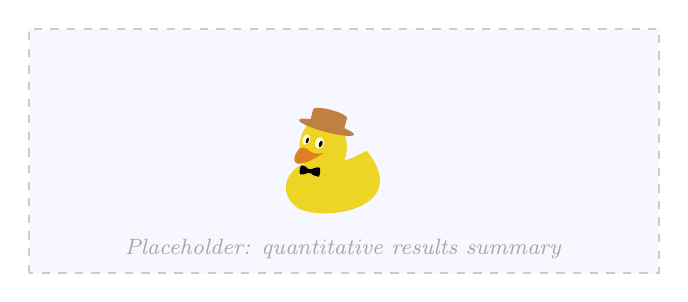
\begin{tikzpicture}
    \fill[blue!3] (-0.5,-0.3) rectangle (7.5,2.8);
    \draw[thick, gray!40, dashed] (-0.5,-0.3) rectangle (7.5,2.8);
    \duck[xshift=2.7cm, yshift=0.4cm, scale=0.6, hat, bowtie]
    \node[gray!70] at (3.5, 0) {\footnotesize\textit{Placeholder: quantitative results summary}};
  \end{tikzpicture}
  \caption{Learned uncertainty improves spatial perception across modalities and platforms.
  (a) Metrics-aware visual covariance yields robust odometry on diverse stereo sequences.
  (b) Learned IMU uncertainty reduces drift in GPS-denied environments.
  (c) Uncertainty-guided quantization and token merging enable real-time deployment on edge hardware.}
  \label{fig:results}
\end{figure}

\section{Future Work}

Building on learned uncertainty for odometry and fusion, my future research pursues three directions that broaden the scope from estimation to deployment, memory, and resilience.

\textbf{Efficient Embodied Deployment.}
Spatial perception must ultimately run on the robots themselves.
While our quantization and token merging work demonstrates that learned models can be compressed with minimal accuracy loss, a deeper challenge remains: co-designing uncertainty estimation with hardware-aware architectures so that perception adapts its compute budget in real time based on scene complexity.
I aim to develop uncertainty-aware perception systems that automatically trade off fidelity and latency, enabling always-on spatial AI on power-constrained embodied platforms, from handheld devices to aerial robots.

\textbf{Spatial Memory with Semantic Understanding.}
Current SLAM systems build geometric maps that lack the semantic richness required for long-horizon tasks.
I plan to extend learned uncertainty into a spatial memory that jointly encodes geometry, semantics, and language-grounded embeddings, enabling robots to answer queries such as ``where did I last see the red toolbox?'' and to reason about scene changes over time.
By integrating vision-language representations with uncertainty-aware mapping, this spatial memory will support task planning, object retrieval, and human-robot interaction across repeated missions in evolving environments.

\textbf{Robustness in Extreme Environments.}
Spatial perception research has largely focused on urban and indoor settings, yet some of the most impactful applications lie in extreme and resource-limited domains: subterranean rescue, deep-sea exploration, and planetary surface operations.
These environments impose severe constraints, including degraded or absent GPS, limited communication, harsh lighting, and strict power budgets.
I aim to leverage learned uncertainty as the mechanism that allows perception systems to degrade gracefully rather than fail catastrophically, adapting sensor fusion strategies and compute allocation to maintain safe operation when conditions push beyond the training distribution.

Together, these directions advance toward spatial perception that is not only accurate but also deployable, semantically rich, and resilient---equipping robots to operate reliably in the environments that matter most.

\bibliographystyle{plainnat}
\bibliography{references}

\end{document}
